\documentclass{article}
\usepackage{graphicx} % Required for inserting images
\usepackage[margin=1in]{geometry}
\usepackage{amsmath}
\usepackage{amsthm}
\usepackage{amssymb}
\usepackage{amsfonts}
\usepackage{verbatim}
\usepackage{tikz}
\usepackage{xcolor}

\title{Homework 1: Report}
\author{Dante Buhl}


\DeclareMathOperator{\cond}{cond}
\DeclareMathOperator{\vecspan}{span}
\DeclareMathOperator{\sign}{sign}

\begin{document}

\newcommand{\bs}[1]{\boldsymbol{#1}}
\newcommand{\bmp}[1]{\begin{minipage}{#1\textwidth}}
\newcommand{\emp}{\end{minipage}}
\newcommand{\R}{\mathbb{R}}
\newcommand{\C}{\mathbb{C}}
\newcommand{\N}{\mathcal{N}}
\newcommand{\I}{\mathrm{I}}
\newcommand{\K}{\bs{\mathrm{K}}}
\newcommand{\m}{\bs{\mu}_*}
\newcommand{\s}{\bs{\Sigma}_*}
\newcommand{\dt}{\Delta t}
\newcommand{\tr}[1]{\text{Tr}(#1)}
\newcommand{\Tr}[1]{\text{Tr}(#1)}

\maketitle



\begin{enumerate}
    
\item Log into Hummingbird and Lux

\begin{center}

    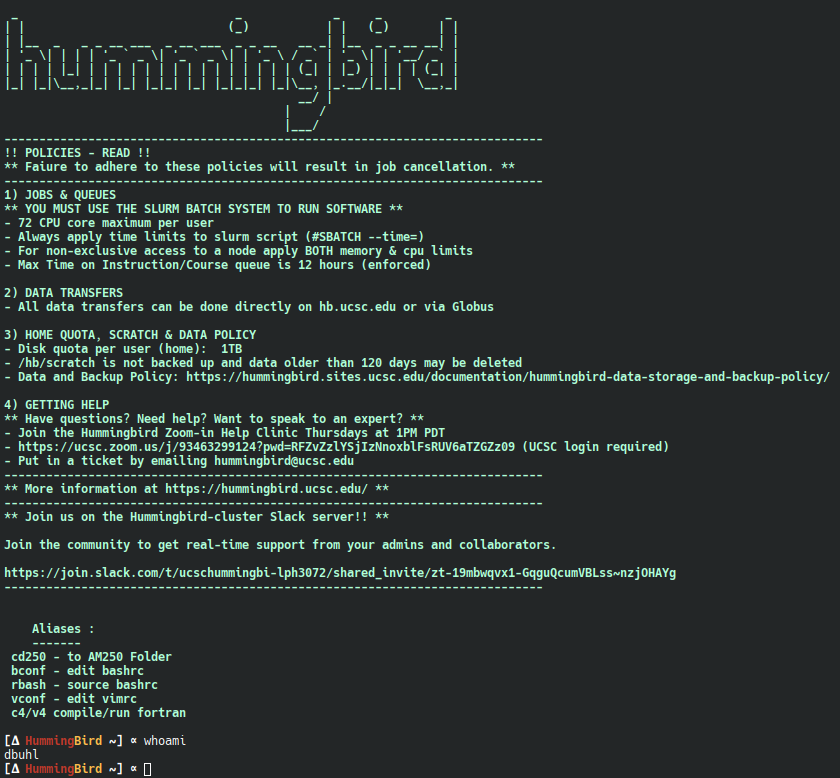
\includegraphics[width=0.7\textwidth]{../hummingbird.png}

\end{center}
 
\item Description of a Top500 Machine. 

    I chose Expanse for the machine to do my report on. I use expanse several times a week so it made sense to become a little more familiar with it. Here are the details.
    \begin{itemize}
        \item Name: Expanse
        \item Location: San Diego Supercomputing Center
        \item Number of Nodes, processors per node, total num of processors: 732, 128, 93,696
        \item Clock Speed of Chips: 2.25 GHz
        \item Flops/processor, total flops: 4608 GFlops, 431.76 PFlops
        \item Memory per processor, total memory: 2 GB, 187 TB
        \item Architecture Type: SIMD, (this really depends on what you are running on it)
        \item Interconnect Type: Mellanox HDR Infiniband
        \item Use: Scientific Research, MY RESEARCH, Fluid Dynamics :)
        \item Anything Special: Its located in California, used to be in the top 200 of machines but its growing a little outdated (EVEN THOUGH IT WAS MADE IN DURING THE PANDEMIC! Its only been 4 years and its been superceeded many times). 
    \end{itemize}

\item Describe something you do in parallel. 

    My routine when I get home is often very similar and it involves me doing things in parallel. Usually the first thing I do is put my backpack down and then turn on my computer. While my computer takes a minute or two to boot up, I press the button on my desk to move it into the standing position, and while the computer boots and my desk lifts up, I take my lunch tupperware to the sink in the kitchen. When I get back the computer is booted and in the position I like. Then I'll put in my password and while the computer brings me to my desktop, I'll put on my headset. Then I open 3 applications all at once. First my terminal, to update any software. Then while its updating, I open Chrome and navigate to my email. Then while my email loads, I go onto Discord and see if I have any new messages. Then I go back to my terminal check if its done, proceed to check my email, and then find something to do. 
   
\end{enumerate}


\end{document}
